\documentclass[12pt,letterpaper]{report}
\usepackage[margin=1in,includeheadfoot]{geometry}
\usepackage[hidelinks,bookmarksnumbered]{hyperref}
\usepackage[figure,table]{hypcap}
\usepackage[nottoc]{tocbibind}
\usepackage[titletoc]{appendix}
\usepackage[utf8]{inputenc}
\usepackage[T1]{fontenc}
\usepackage{todonotes}

\usepackage{fancyhdr}
\pagestyle{fancy}
\fancyhf{}
\rhead{\textit{\leftmark}}
\cfoot{\thepage}
\renewcommand{\headrulewidth}{0pt}

\usepackage[backend=biber]{biblatex}
\addbibresource{references.bib}

\usepackage{graphicx}
\graphicspath{ {images/} }

\usepackage{setspace}
\onehalfspacing

\usepackage{datetime}
\newdateformat{monthyeardate}{\monthname[\THEMONTH] \THEYEAR}
\newdateformat{yeardate}{\THEYEAR}

\usepackage{sectsty}
\chapterfont{\vspace*{-14.88mm}\large\sc\centering}
\chaptertitlefont{\centering}
\subsubsectionfont{\centering}

%----------------
% Title Page
%----------------
\begin{document}

\begin{titlepage}
	\begin{center}
		\vspace*{1in}
		
		\Huge
		Thesis Title
		
		\vfill
		
		\large
		Cheuk Chuen Siow\\
		School of Computer Science\\
		McGill University, Montréal
		
		\vfill
		
		\monthyeardate\today
		
		\vfill
		
		A thesis submitted to McGill University in partial fulfillment of the requirements for the degree of Master of Science in Computer Science
		
		\vfill
		
		\textcopyright{} Cheuk Chuen Siow \yeardate\today
		
		\vspace*{1in}
	\end{center}
\end{titlepage}

%----------------
% Front Matter
%----------------
\clearpage
\pagenumbering{roman}
\setcounter{page}{2}

\chapter*{Abstract}
\addcontentsline{toc}{chapter}{Abstract}



\clearpage

\chapter*{Abrégé}
\addcontentsline{toc}{chapter}{Abrégé}



\clearpage

\chapter*{Acknowledgements}
\addcontentsline{toc}{chapter}{Acknowledgements}



\clearpage

\chapter*{Preface}
\addcontentsline{toc}{chapter}{Preface}



% Content
\renewcommand{\contentsname}{Table of Contents}
\tableofcontents
\listoffigures
\listoftables

\clearpage
\pagenumbering{arabic}

%----------------
% Main Body
%----------------
\chapter{Introduction}
% !TEX root = ../thesis.tex

Since 1960s, software development has been evolving rapidly to address the increasing demands of complex software. The complexity of modern software brings about difficulties in developing and maintaining quality software. Software engineering as a discipline ensures that developers follow a systematic production of software, by applying best practices to maximize quality of deliverables and minimize time-to-market. Various methodologies exist through the efforts of active research by theorists and practitioners, but the core of software development process typically consists of the following six phases---requirements gathering, design, implementation, testing, deployment, and maintenance.

Conceptual models help illustrates complex systems with a simple framework by creating abstractions to alleviate the amount of complexity. Hence, the use of models is progressively recommended in representing a software system. This simplifies the process of design, maximizes compatibility between different platforms, and promotes communication among stakeholders. Model-Driven Engineering (MDE) technologies offer the means to represent domain-specific knowledge within models, allowing modelers to express domain concepts effectively~\cite{schmidt2006model}. MDE advocates using the best modeling formalism that expresses relevant design intent declaratively at each level of abstraction. During development, we can use models to describe different aspects of the system vertically, in which the models are refined from higher to lower levels of abstraction through model transformation. At the lowest level, models use implementation technology concepts, and appropriate tools can be used to generate code from these platform-specific models~\cite{sendall2003model}.

Modularity is key in designing computer programs that are extensible and easily maintainable, but concerns that are crosscutting and more scattered in the implementation are more likely to cause defects~\cite{eaddy2008crosscutting}. This poses obstacles for MDE because modeling such crosscutting concerns in a modular way is difficult from an object-oriented standpoint. Furthermore, reusability is also a main factor in allowing developers to leverage reusable solutions such as libraries and frameworks provided for a given programming language, thereby improving the development speed without having to implement existing software components from first principles. Model reuse is still in its early stage, but modeling libraries are emerging as well~\cite{france2012repository}.

Concern-Oriented Reuse (CORE) is a new software development paradigm or approach that puts reuse at the forefront of software development~\cite{alam2013concern}. In CORE, software development is structured around modules called \emph{concerns} that provide a variety of reusable solutions for recurring software development issues. Techniques from MDE, Software Product Lines (SPL) engineering, and software composition (in particular feature-orientation and aspect-orientation) allow concerns to form modular units of reuse that encapsulate a set of software development artifacts, i.e., models and code, during software development in a versatile, generic way.

The main premise of CORE is that recurring development concerns are made available in a concern library, which eventually should cover most recurring software development needs. Similar to class libraries in modern programming languages, this library should grow as new development concerns emerge, and existing concerns should continuously evolve as alternative architectural, algorithmic, and technological solutions become available. Applications are built by reusing existing concerns from the library whenever possible, following a well-defined reuse process supported by clear interfaces. To generate an executable in which concerns exhibit intricate crosscutting structure and behavior, CORE relies on additive software composition techniques, feature-oriented technology, and aspect-oriented technology.

Currently, CORE only supports modelling notations that are used at the design phase~\cite{kienzle2010aspect}. In order to fully integrate CORE with MDE, other development phases should also be supported. We are interested in adding support for requirements modeling languages to CORE, so that requirements modellers too can benefit from advanced modularization and reuse support. We chose to concentrate on the User Requirements Notation (URN), which sets the standard as a visual notation for modeling and analyzing requirements~\cite{amyot2002urn}. URN formalizes and integrates two complementary languages: (i) Goal-oriented Requirements Language (GRL) to describe non-functional requirements as intentional elements, and (ii) Use Case Map (UCM) to describe functional requirements as causal scenarios. GRL and UCM are used to capture goal and scenario models, respectively. Since CORE already supports the use of goal models to analyze the impact of choosing features~\cite{alam2013concern}, this thesis focuses on integrating scenario models with the concepts of CORE.

\section{Contributions}

This thesis advances the state-of-the-art in modeling by proposing a complete solution for augmenting the UCM modeling notation with CORE capabilities, resulting in a variant of UCM---Concern-Oriented Use Case Maps (CoUCM). Specifically, the thesis makes the following contributions:

\begin{itemize}

\item A metamodel for CoUCM that extends the CORE metamodel, thus formalizing the integration of the CORE concepts into the UCM language.

\item A CORE-compatible weaving algorithm for CoUCMs that takes as an input two CoUCM models and produces a composed CoUCM model. This makes it possible for requirements engineers to modularize scenarios according to concern features (i.e., a weaving algorithm compatible with CORE extension) as well as to reuse existing scenarios when creating new ones (i.e., compatible with the CORE reuse mechanism).

\item An implementation of the proposed CoUCM metamodel and weaving algorithm in TouchCORE, serving as a proof of concept validation.

\item A demonstration of the expressiveness and reuse potential of CoUCMs by means of an \emph{Authentication} concern and an \emph{Online Payment} concern, and two \emph{Workflow Patterns} case studies.

\end{itemize}

\section{Thesis Outline}

The remainder of this thesis is structured as follows. Chapter~\ref{ch:2} offers background information on CORE and UCM, as well as presents existing modeling techniques closely related to our work. Chapter~\ref{ch:3} details the integration of CORE with UCM, namely the CoUCM meta model and the different CoUCM weaving algorithms. Chapter~\ref{ch:4} validates the proposed meta model
and weaving algorithms by presenting some details of the TouchCORE implementation. Finally, Chapter~\ref{ch:5} concludes the thesis and discusses possible future work.


\chapter{Background}
First paragraph opens with URN and its components.

\section{Use Case Map (UCM)}

This section describes UCM in detail.

\section{Concern-oriented Reuse (CORE)}

This section describes CORE in detail.

\subsection{Reusable Aspect Models (RAM)}

\section{Overview of Relevant Modeling Tools}

Literature review.

\section{Motivation}

Build on the motivation of having UCM as an additional model for TouchCORE.

\subsection{UCM in the Context of CORE}

Weaving, extending, and reusing UCM concern models.

Last paragraph leads to implementation chapter.


\chapter{Methods}
\todo[inline]{How about as a title: Adding Support for Use Case Maps to CORE}

\todo[inline]{Then talk about (or remind the reader about) motivation, then detail that there needs to be support in the metamodel, the concrete syntax, and the weaving algorithm. It could also be possible to not talk about the concrete syntax here, but in the next chapter (the implementation). This chapter really describes the conceptual work of adding UCMS to CORE.}

\section{UCM Metamodel}

\subsection{Abstract Syntax}

\subsection{Concrete Syntax}

\todo[inline]{Maybe move this to the next chapter... To discuss}

\section{Weaver}

\todo[inline]{Again, maybe we need a short intro here. I assume there is also a common algorithm to extensions and reuses, or are they completely separate?}

\subsection{Model Extension}

\subsection{Model Reuse}


\chapter{Results}
\todo[inline]{Maybe a good title would be "UCM Implementation in TouchCORE"?}

\todo[inline]{Then again we need an intro to the chapter explaining what is to come.}

\section{Scenario Model in TouchCORE}

Lots of figures here.

\section{Model Weaving with UCMs}

Lots of illustrations here.



\chapter{Discussion}
\todo[inline]{Maybe this chapter can be called validation? In a sense, you are validating your proposed approach with case studies (1) and then showing that you can cover the workflow patterns (2). That's pretty substantial for a masters thesis}

\todo[inline]{Again, a short intro is needed to explain the 2 forms of validation}

\section{Case Study}

\subsection{Authentication}

\subsection{Online Payment}

\section{Workflow Patterns}


\chapter{Conclusion}
\todo[inline]{I would first put the conclusion, and then the future work}

\section{Future Work}

Remaining tasks such as components, path drawing, validation, semantics, etc.

\section{Summary}

Recap of thesis: what I did so far and what can the tool achieve.


%----------------
% End Matter
%----------------
\begin{appendices}

\chapter{Complete Authentication Model}
\section{CORE Metamodel}

\begin{figure}[h]
	\centering
	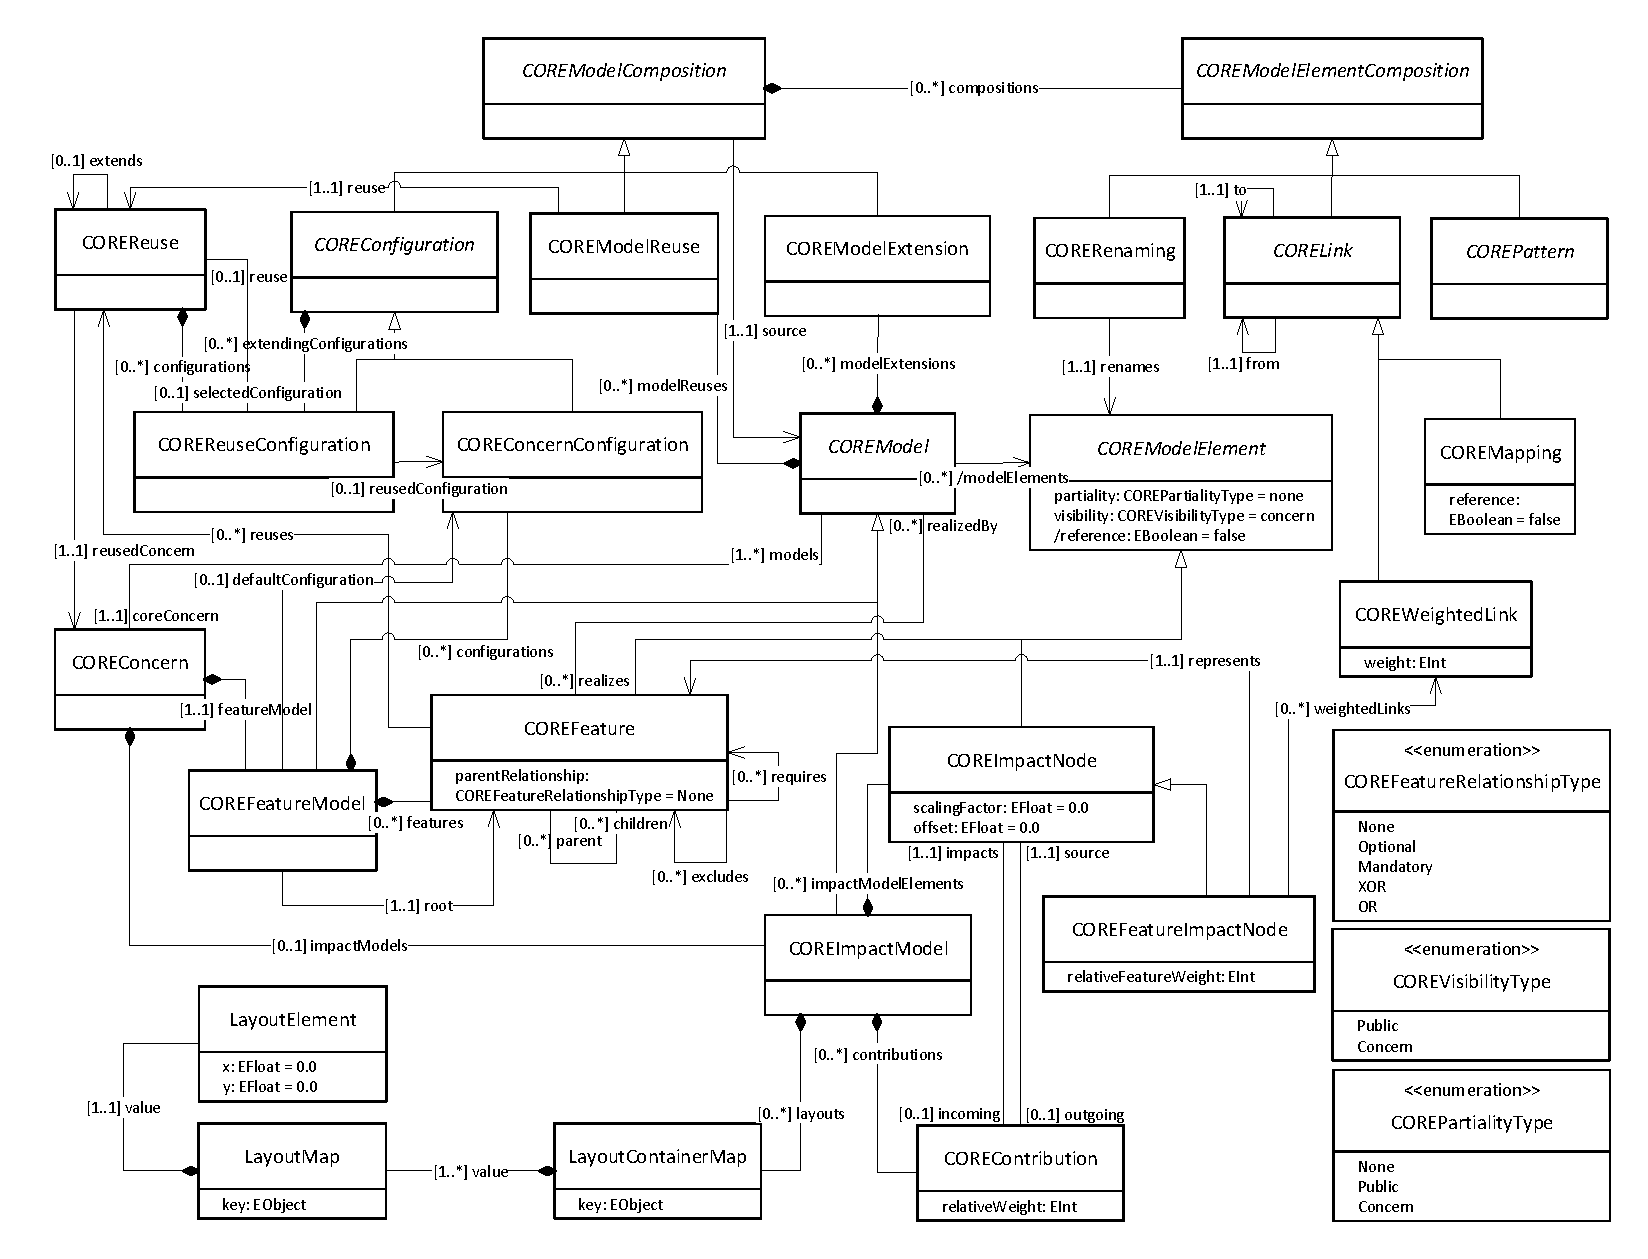
\includegraphics[scale=0.59]{fig_a_1.pdf}
	\caption{Abstract grammar: CORE metamodel overview}
	\label{fig:a.1}
\end{figure}

\section{UCM Metamodel}

\begin{figure}[h]
	\centering
	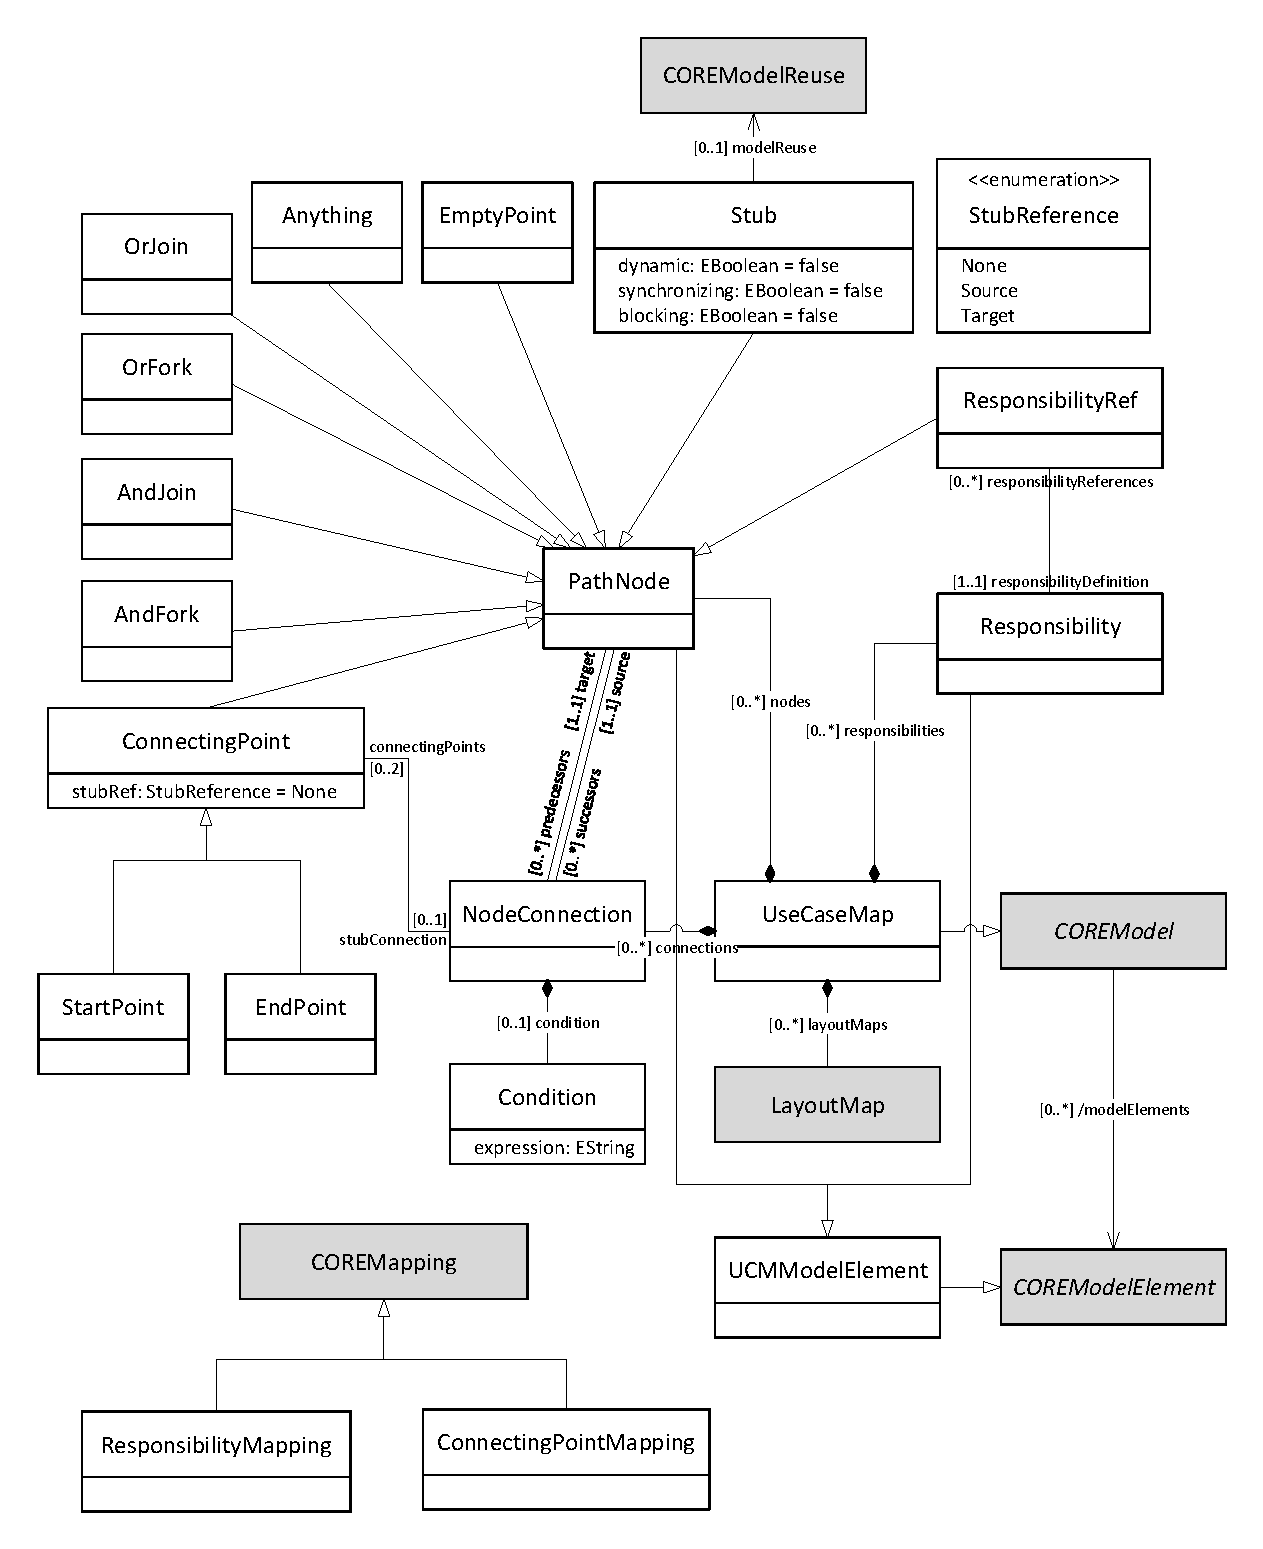
\includegraphics[scale=0.53]{fig_a_2.pdf}
	\caption{Abstract grammar: UCM metamodel overview}
	\label{fig:a.2}
\end{figure}


\chapter{Complete Online Payment Model}
\section{Authentication Model}

\section{Online Payment Model}


\end{appendices}

\renewcommand\bibname{References}
\printbibliography[heading=bibintoc]

\end{document}
